\documentclass{sig-alternate}
%\usepackage[latin1]{inputenc} % Windows
\usepackage[utf8x]{inputenc} % Linux (unicode package needed)
% \usepackage[applemac]{inputenc} % Mac

\usepackage{url}

\usepackage{balance}

\usepackage{graphicx}
\usepackage{caption}
\usepackage{subcaption}
\usepackage{hyperref}

\usepackage{xcolor}
\usepackage{color}

\newcommand{\brand}[1]{\textbf{\tt #1}}

\usepackage{enumitem}
\setlist[description]{leftmargin=\parindent}

\definecolor{editorGray}{rgb}{0.95, 0.95, 0.95}
\definecolor{editorOcher}{rgb}{1, 0.5, 0} % #FF7F00 -> rgb(239, 169, 0)
\definecolor{editorGreen}{rgb}{0, 0.5, 0} % #007C00 -> rgb(0, 124, 0)
\colorlet{punct}{red!60!black}
\definecolor{background}{HTML}{FEFEFE}
\definecolor{delim}{RGB}{20,105,176}
\colorlet{numb}{magenta!60!black}

\usepackage{upquote}
\usepackage{listings}
\lstdefinelanguage{JavaScript}{
  morekeywords={typeof, new, true, false, catch, function, return, null, catch, switch, var, if, in, while, do, else, case, break},
  morecomment=[s]{/*}{*/},
  morecomment=[l]//,
  morestring=[b]",
  morestring=[b]'
}

\lstdefinelanguage{HTML5}{
        language=html,
        sensitive=true, 
        alsoletter={<>=-},
        otherkeywords={
        % HTML tags
        <html>, <head>, <title>, </title>, <meta, />, </head>, <body>,
        <canvas, \/canvas>, <script>, </script>, </body>, </html>, <!, html>, <style>, </style>, ><
        },  
        ndkeywords={
        % General
        =,
        % HTML attributes
        charset=, id=, width=, height=,
        % CSS properties
        border:, transform:, -moz-transform:, transition-duration:, transition-property:, transition-timing-function:
        },  
        morecomment=[s]{<!--}{-->},
        tag=[s]
}

\lstset{%
    % Basic design
    backgroundcolor=\color{white},
    basicstyle={\scriptsize\ttfamily},   
    frame=l,
    % Line numbers
    xleftmargin={0.75cm},
    numbers=left,
    stepnumber=1,
    firstnumber=1,
    numberfirstline=true,
    % Code design   
    keywordstyle=\color{blue}\bfseries,
    commentstyle=\color{darkgray}\ttfamily,
    ndkeywordstyle=\color{editorGreen}\bfseries,
    stringstyle=\color{delim},
    % Code
    language=HTML5,
    alsolanguage=JavaScript,
    alsodigit={.:;},
    tabsize=2,
    showtabs=false,
    showspaces=false,
    showstringspaces=false,
    extendedchars=true,
    breaklines=true,        
    % Support for German umlauts
    literate=%
    {Ö}{{\"O}}1
    {Ä}{{\"A}}1
    {Ü}{{\"U}}1
    {ß}{{\ss}}1
    {ü}{{\"u}}1
    {ä}{{\"a}}1
    {ö}{{\"o}}1
}

\lstdefinelanguage{json}{
    basicstyle=\scriptsize\ttfamily,
    % numbers=left,
    % numberstyle=\scriptsize,
    % stepnumber=1,
    % numbersep=8pt,
    % showstringspaces=false,
    % breaklines=true,
    % frame=lines,
    backgroundcolor=\color{background},
    literate=
     *{0}{{{\color{numb}0}}}{1}
      {1}{{{\color{numb}1}}}{1}
      {2}{{{\color{numb}2}}}{1}
      {3}{{{\color{numb}3}}}{1}
      {4}{{{\color{numb}4}}}{1}
      {5}{{{\color{numb}5}}}{1}
      {6}{{{\color{numb}6}}}{1}
      {7}{{{\color{numb}7}}}{1}
      {8}{{{\color{numb}8}}}{1}
      {9}{{{\color{numb}9}}}{1}
      {:}{{{\color{punct}{:}}}}{1}
      {,}{{{\color{punct}{,}}}}{1}
      {\{}{{{\color{delim}{\{}}}}{1}
      {\}}{{{\color{delim}{\}}}}}{1}
      {[}{{{\color{delim}{[}}}}{1}
      {]}{{{\color{delim}{]}}}}{1},
}

\begin{document}

% Copyright
\setcopyright{acmcopyright}
%\setcopyright{acmlicensed}
%\setcopyright{rightsretained}
%\setcopyright{usgov}
%\setcopyright{usgovmixed}
%\setcopyright{cagov}
%\setcopyright{cagovmixed}


% DOI
\doi{10.475/123_4}

% ISBN
\isbn{123-4567-24-567/08/06}

%Conference
\conferenceinfo{DocEng2015}{Sep 8--11, 2015, Lausanne, Switzerland}

\acmPrice{\$15.00}

\title{x-project: a document-oriented toolkit to design and implement Web Applications based on HTML5 Web Components}

\numberofauthors{4} 
\author{
\alignauthor
Andrea D'Amelio\\
  \affaddr{Universit\`a Roma Tre}\\
  \affaddr{Dipartimento di Ingegneria}\\
  \affaddr{Universit\`a Roma Tre}\\
  \affaddr{Rome, Italy}\\
  \email{damelio@ing.uniroma3.it}
\alignauthor
Enrico Marino\\
  \affaddr{Universit\`a Roma Tre}\\
  \affaddr{Dipartimento di Ingegneria}\\
  \affaddr{Universit\`a Roma Tre}\\
  \affaddr{Rome, Italy}\\
  \email{marino@ing.uniroma3.it}
\and
\alignauthor
Tiziano Sperati\\
  \affaddr{Universit\`a Roma Tre}\\
  \affaddr{Dipartimento di Ingegneria}\\
  \affaddr{Universit\`a Roma Tre}\\
  \affaddr{Rome, Italy}\\
  \email{sperati@ing.uniroma3.it}
\alignauthor
Federico Spini\\
  \affaddr{Universit\`a Roma Tre}\\
  \affaddr{Dipartimento di Ingegneria}\\
  \affaddr{Universit\`a Roma Tre}\\
  \affaddr{Rome, Italy}\\
  \email{spini@ing.uniroma3.it}
}

\maketitle

\begin{abstract}
Lorem ipsum dolor sit amet, consectetur adipisicing elit, sed do eiusmod
tempor incididunt ut labore et dolore magna aliqua. Ut enim ad minim veniam,
quis nostrud exercitation ullamco laboris nisi ut aliquip ex ea commodo
consequat. Duis aute irure dolor in reprehenderit in voluptate velit esse
cillum dolore eu fugiat nulla pariatur. Excepteur sint occaecat cupidatat non
proident, sunt in culpa qui officia deserunt mollit anim id est laborum.

Lorem ipsum dolor sit amet, consectetur adipisicing elit, sed do eiusmod
tempor incididunt ut labore et dolore magna aliqua. Ut enim ad minim veniam,
quis nostrud exercitation ullamco laboris nisi ut aliquip ex ea commodo
consequat. Duis aute irure dolor in reprehenderit in voluptate velit esse
cillum dolore eu fugiat nulla pariatur. Excepteur sint occaecat cupidatat non
proident, sunt in culpa qui officia deserunt mollit anim id est laborum.

\end{abstract}


%
% The code below should be generated by the tool at
% http://dl.acm.org/ccs.cfm
% Please copy and paste the code instead of the example below. 
%

\begin{CCSXML}
<ccs2012>
<concept>
<concept_id>10002951.10003260.10003282</concept_id>
<concept_desc>Information systems~Web applications</concept_desc>
<concept_significance>500</concept_significance>
</concept>
<concept>
<concept_id>10010405.10010476.10010479</concept_id>
<concept_desc>Applied computing~Cartography</concept_desc>
<concept_significance>500</concept_significance>
</concept>
<concept>
<concept_id>10010405.10010497.10010510.10010514</concept_id>
<concept_desc>Applied computing~Format and notation</concept_desc>
<concept_significance>500</concept_significance>
</concept>
<concept>
<concept_id>10010520.10010521.10010537.10010538</concept_id>
<concept_desc>Computer systems organization~Client-server architectures</concept_desc>
<concept_significance>300</concept_significance>
</concept>
<concept>
<concept_id>10010520.10010570.10010574</concept_id>
<concept_desc>Computer systems organization~Real-time system architecture</concept_desc>
<concept_significance>300</concept_significance>
</concept>
</ccs2012>
\end{CCSXML}

\ccsdesc[500]{Information systems~Web applications}
\ccsdesc[500]{Applied computing~Cartography}
\ccsdesc[500]{Applied computing~Format and notation}
\ccsdesc[300]{Computer systems organization~Client-server architectures}
\ccsdesc[300]{Computer systems organization~Real-time system architecture}

%
% End generated code
%

%
%  Use this command to print the description
%
\printccsdesc



\section{Introduction}
Lorem ipsum dolor sit amet, consectetur adipisicing elit, sed do eiusmod
tempor incididunt ut labore et dolore magna aliqua. Ut enim ad minim veniam,
quis nostrud exercitation ullamco laboris nisi ut aliquip ex ea commodo
consequat. Duis aute irure dolor in reprehenderit in voluptate velit esse
cillum dolore eu fugiat nulla pariatur. Excepteur sint occaecat cupidatat non
proident, sunt in culpa qui officia deserunt mollit anim id est laborum.


Section 2 presents the context where \brand{x-project} is positioned, overviewing the CMS evolution; section 3 introduces \brand{x-project}, its philosophy and architecture. Section 4 shows a case study in which is implemented a blog using x-project toolkit. Finally, section 5 draws conclusions.


\section{Evolution of CMSs}
One generally accepted definition of Content Management System is: a system that lets you apply management principles to content.

It is simple to elicit an evolutionary path in the history of management systems whose milestones are identifiable in \emph{Joomla!}, \emph{Wordpress} and \emph{KeystoneJS}.

Alongside these milestones entire constellations of analogous experiences popped up, but we considered them not relevant since they borrowed main features and constitutive approaches from cited ones. 

Starting from \emph{Joomla!}, a framework that drove in the engineering into the world of web content management. Joomla! powers more than 2,7\% of the largest 1,000,000 web sites in the world \cite{usage-cms}. Anyway, nowadays, \emph{Joomla!} results unwieldy and, due to its monolithic approach, not complied to current web features.

\emph{Wordpress}, instead is used by more than 23.3\% of the top 10 million websites (as of January 2015) \cite{usage-cms}. Wordpress develop CMS’s idea, driving in the intention to use CMSs to build Web Application. Wordpress, with its plugin, aims to limber user experience. The availability of more than 37,000 plugins, because it lets to create sites to non-experts too.
Anyway, further customizations, other than the ones introduced by plugins, are difficult to deploy due to loosely code engeneering of this tool.

Finally, \emph{KeystoneJs} stand in the last position. Minimal and agile, KeystoneJS, embody the new era of the CMS, letting the user to make his own personal web application.

In the spite of focusing on very minimal features, a mention goes to Ghost, a non-profit, open source blogging Node.js based platform, which represents a transversal experience, although minimal brings a new light way to blogging.

Eventually, \brand{x-project}, for the reasons the will be clear in the remaining of this paper, could be thought as the last standing in this path of decreasing monolithic approach and increasing customization and code engineering.



\section{x-project toolkit}
\brand{x-project} is a set of libraries and API-centric HTML5 Web Components based Web Application and CMS framework.



% \subsection{Philosophy}
``Everything is an element'', even an AJAX request. Every part of the website is encapsulated inside an element. Even functional components such as HTTP services (AJAX calls), pages and routing logic are encapsulated inside elements. We push Web Components' philosophy beyond all limits so that users can reach a very high level of customization and ease of use.

Component-based Software Engineering denotes the process of building software by (re)using pre-built software components. The main benefit of component-based software is the ``time-to-market'' \cite{4773208}, thus reducing the cost of developing the software. A software component is a unit of composition with contractually specified interfaces and explicit context dependencies. 
Additionally, a component is a software element that conforms to a component model and can be independently deployed and composed \cite{Heineman:2001:CSE:379381}. 
Component based software is developed interconnecting building blocks, therefore, a high degree of reusability and modularity is achieved by this type of applications \cite{914739}. 



\subsection{Architecture}
\brand{x-project} architecture is client-server.
The full technology stack is JavaScript based.

Server-side is based on Node.js.

\begin{description}
\itemsep1pt\parskip0pt\parsep0pt
        \item[Node.js] (\url{http://nodejs.org}) is a platform built on Chrome's JavaScript runtime for easily building fast, scalable network applications.
        \item[Express.js] (\url{http://expressjs.com}) is a minimal and flexible Node.js web application framework that provides a set of features for web and mobile applications.
        \item[Loopback] (\url{http://loopback.io}) is a set of Node.js modules to develop Web Servers applications. An application interacts with data sources through the LoopBack model API, available locally within Node.js, remotely over REST.
        \item[MongoDB] (\url{https://www.mongodb.org/}) is an open-source document database that provides high performance, high availability, and automatic scaling.
\end{description}


Client-side is based on Web Components.

\begin{description}
\itemsep1pt\parskip0pt\parsep0pt
        \item[Web Components] are a collection of standards which are working their way through the W3C and landing in browsers at the moment. In a nutshell, they allow us to bundle markup and styles into custom HTML elements.
\emph{Custom Elements}\cite{custom-elements}, \emph{HTML Imports}\cite{html-imports}, \emph{HTML Templates}\cite{html-templates}, \emph{Shadow DOM}\cite{shadow-dom}.
        \item[webcomponent.js polyfills] enable Web Components in (evergreen) browsers that lack native support.
Web Components specifications are currently W3C Working Draft, so they aren’t fully supported across all major browsers.
As these technologies are implemented in browsers, the polyfills will shrink to gain the benefits of native implementations. \cite{webcomponents-polyfills} 
        \item[Polymer library] (\url{https://www.polymer-project.org/}) provides a thin layer of API on top of web components (native implementations and their polyfills) and several powerful features, such as custom events and delegation, mixins, accessors and component lifecycle functions, that makes it easier and faster to create Web Components. Similar to \emph{Polymer} are \emph{x-tag} and \emph{Bosonic}.
        \item[iron-elements] \cite{iron-elements} is a library of utility Polymer elements from ajax requests to input elements. 
There are web repositories like \url{http://component.kitchen} and \url{http://customelements.io} that already counts thousands of open source user-contributed custom elements.
\end{description}

% \begin{figure}[!htbp]
% \centering
% 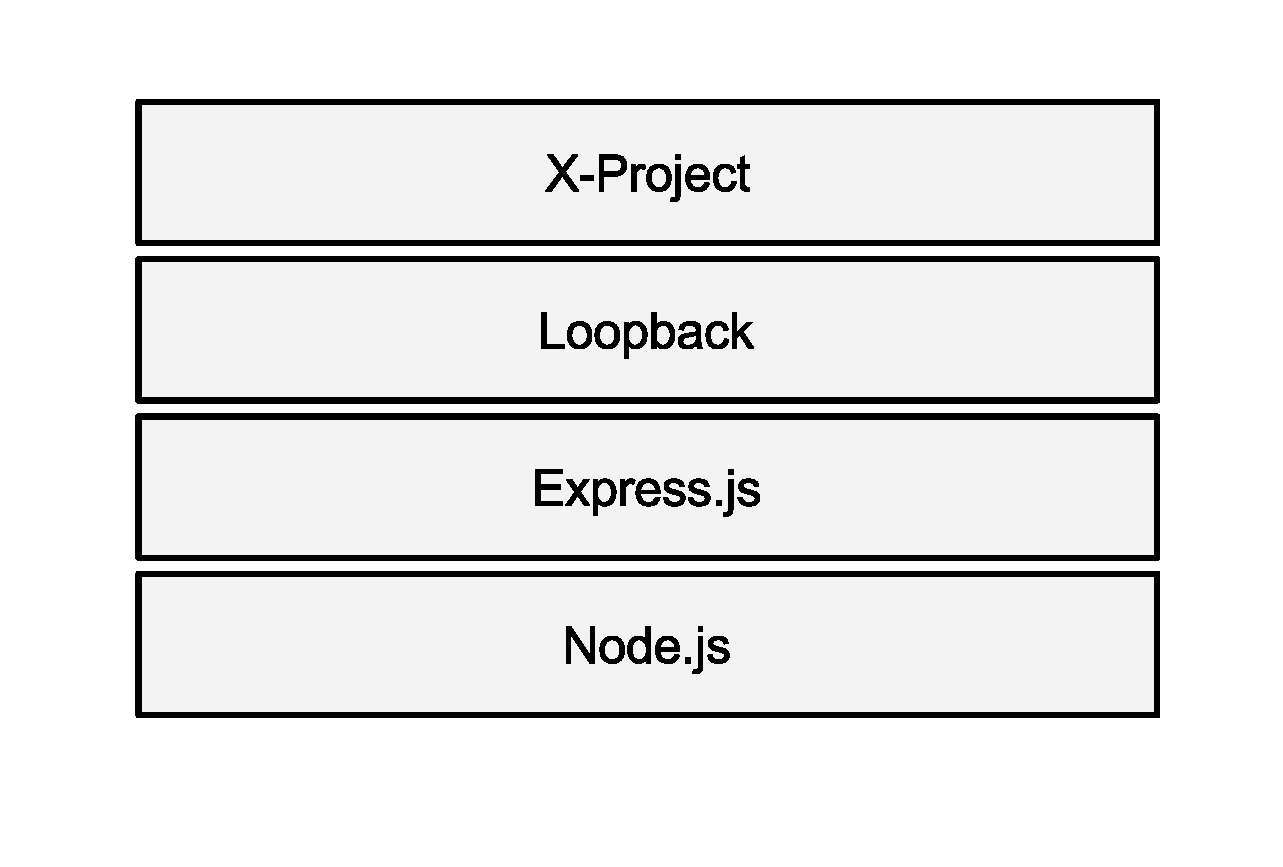
\epsfig{file=images/stack.eps, height=0.2\textwidth}
% \caption{Technology stack}
% \label{fig:tech-stack}
% \end{figure}

% \begin{figure}[!h]
%  \centering
%  \begin{subfigure}[b]{0.53\linewidth}
%  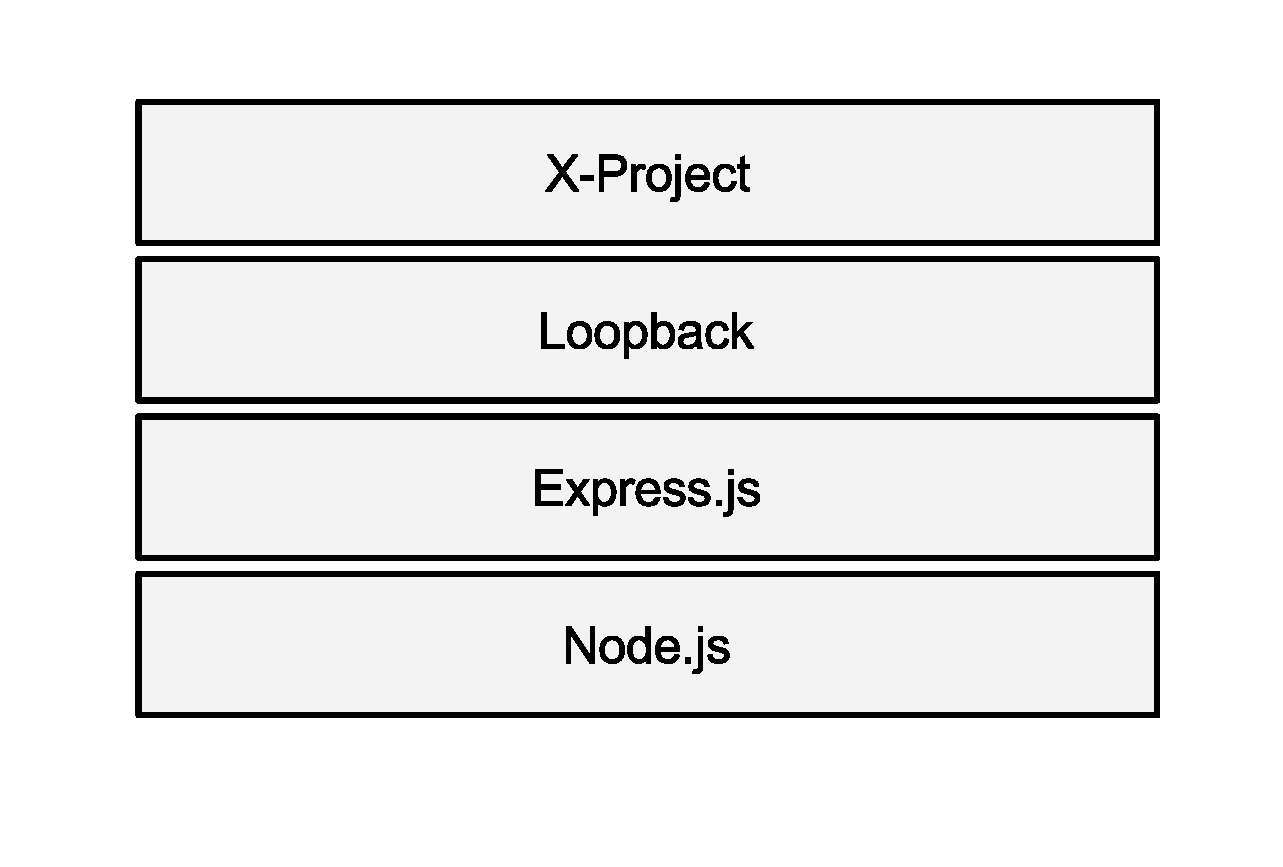
\includegraphics[width=\textwidth]{images/stack.eps} 
%  \caption{Technology stack.}
%  \label{fig:tech-stack}
%  \end{subfigure}
%  ~
%  \begin{subfigure}[b]{0.43\linewidth}
%  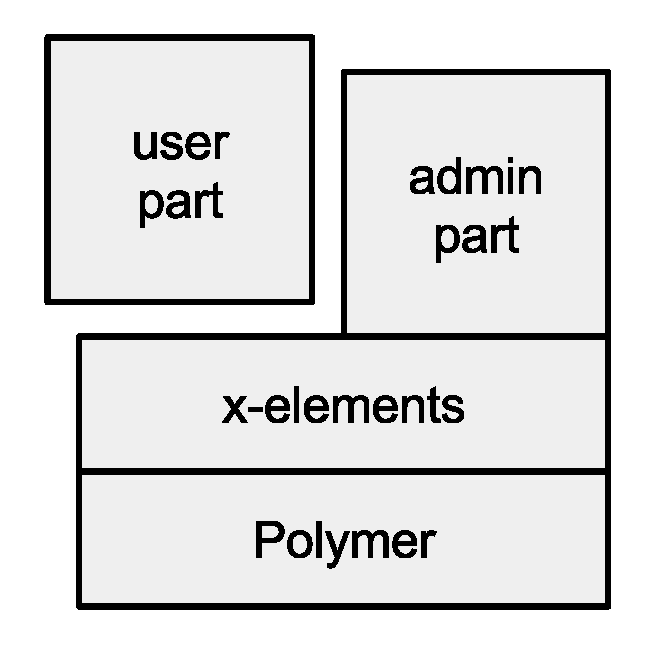
\includegraphics[width=\textwidth]{images/client-arch.eps}
%  \caption{Client-side architecture}
%  \label{fig:client-arch}
%  \end{subfigure}
 
%  % \caption{Office building: 
%  % (a) the schematic plan; 
%  % (b) the simplified 3D model generated for testing on the field 
%  % the indoor mapping project described in this paper.
%  % }
%  % \label{fig:sogei}
% \end{figure}

% \begin{figure}[!htbp]
% \centering
% 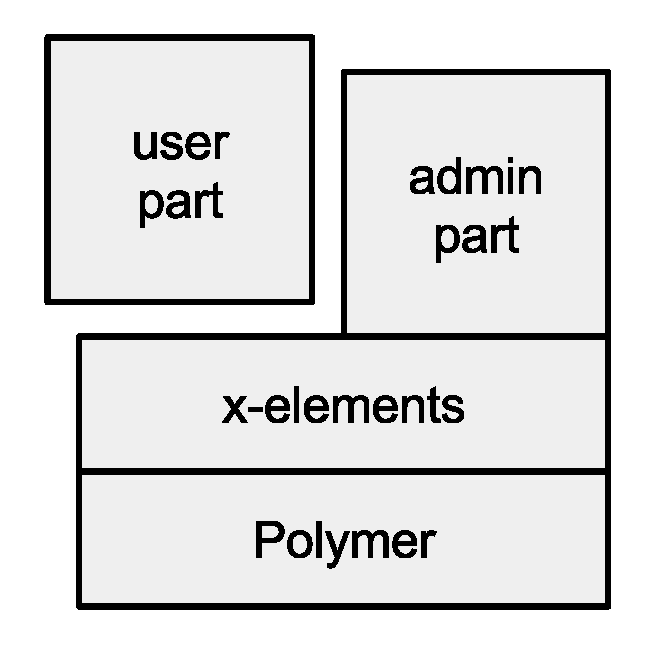
\epsfig{file=images/client-arch.eps, height=0.2\textwidth}
% \caption{Client-side architecture}
% \label{fig:client-arch}
% \end{figure}


\subsection{Server-side}
The Web Application development is document-driven.

To speed up web application development, frameworks mostly rely on external configuration files and less on procedural code \cite{6859693}.


In \brand{x-project}, server-side, the documents that drive the development are the schema of the models of the application.


These are json document. Each document represent a model and has the following fields: the \texttt{name} of the model, the set of \texttt{properties}, the list of \texttt{relations} to others models and the list of \texttt{ACL} (Access Control Layer) rules. 

\brand{x-project} (using Loopback) generates model’s API from the models schemas, to let CRUD operations on models (e.g. a model \texttt{Author} that describe a blog author generates the following HTTP RESTful API: \texttt{GET /api/authors/} to get all authors, \texttt{POST /api/authors/} to add a new author, \texttt{GET /api/authors/:author\_id} and \texttt{PUT /api/authors/:author\_id} to get (or to update) the author with id ``\texttt{author\_id}''. 
Since an blog author have blog posts (its model has a relation one-to-many to model \texttt{Post}) there are also the API to handle author's posts: \texttt{GET /api/authors/:author\_id/posts}, etc.

The API can be extended: the developer can add remote functions to models or add hooks to existing APIs to add behaviour before and/or after the API handler (to preprocess the request and/or postprocess the response).

The API are RESTful, cookie free, signed by authentication token.

\brand{x-project} applications have a built-in model that represent a user, with properties \texttt{username}, \texttt{email} and \texttt{password} for login and the property \texttt{role} used by the ACL module.
By default, only user with role \texttt{admin} can create/update/delete models in the applications.


\subsubsection{Third party services}
\brand{x-project} is designed to be connected to microservices. These tools are accessible extending the Web Application API.

An essential feature of a CMS is media storage (documents, images and videos) \cite{5552271}. 

\brand{x-project} provides a remote storage service implemented as a direct upload module to AWS Amazon S3 storage service. The media to upload don’t pass through the server but are sent directly to AWS using a signed request.
The signature of the request is provided by the module.
The module has to be configured with the AWS bucket settings: bucket name, public and secret keys. 

% \begin{figure}[!htbp]
% \centering
% 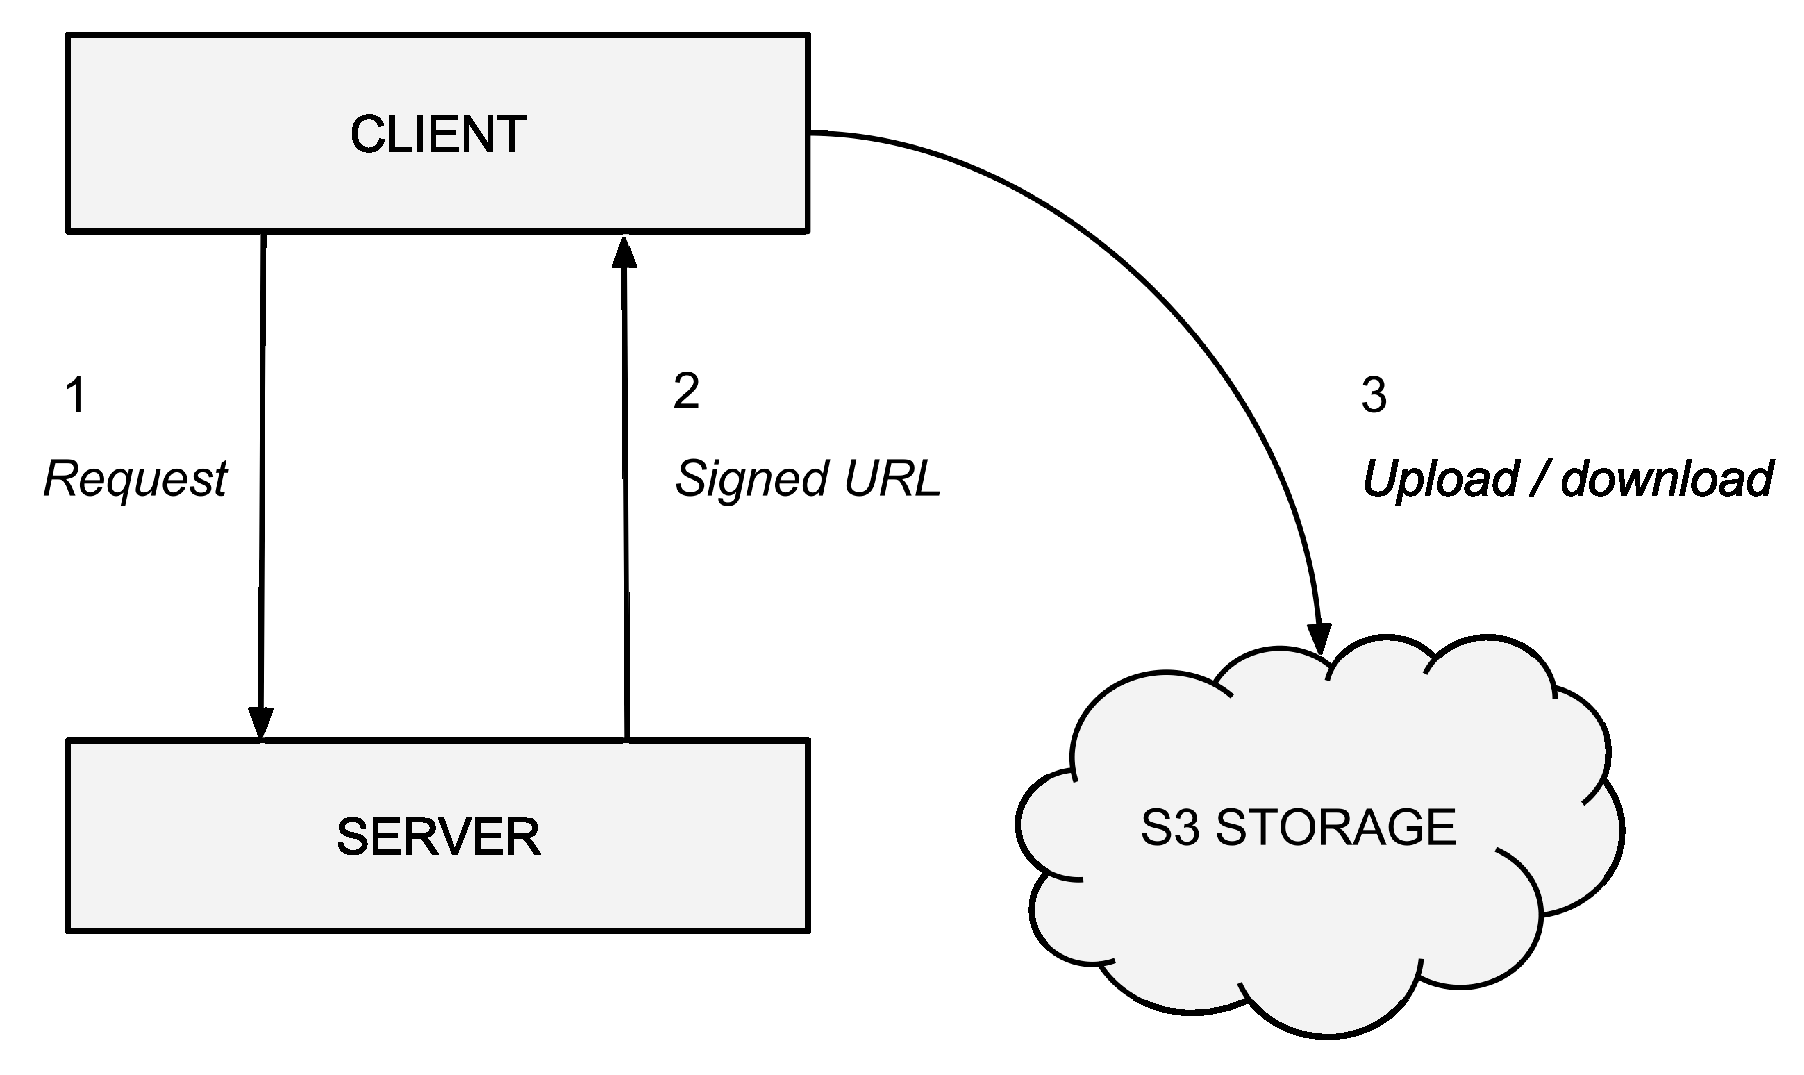
\epsfig{file=images/services.eps, height=0.24\textwidth}
% \caption{Third parties services}
% \label{fig:services}
% \end{figure}


\subsection{Client-side}

Client-side can be divided in two parts: \texttt{admin part} and \texttt{user part}.
\texttt{admin part} is automatically generated from the models schemas. It let the admin to manage (via CRUD operations) the models.
\texttt{user part} depends on the type of the Web Application that has been implemented.
It is the part the final user interact with.

% \begin{figure}[!htbp]
% \centering
% 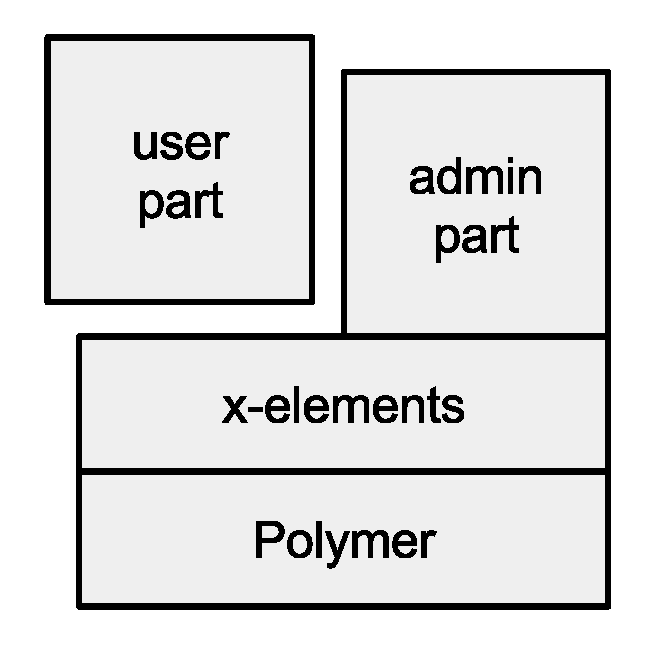
\epsfig{file=images/client-arch.eps, height=0.2\textwidth}
% \caption{Client-side architecture}
% \label{fig:client-arch}
% \end{figure}

\brand{x-project} provide a set of Polymer element for local routing, API requests, User management, forms composition, layout and style. 

\subsubsection{Elements for local routing}
\brand{x-project} provide elements to perform local routing to implement Single Page Application pattern.

\begin{description}
\itemsep1pt\parskip0pt\parsep0pt
        \item[\texttt{<x-router>}] implements local routing based on \emph{HTML5 Push State API}. 
        \item[\texttt{<x-route>}] represents a route-to-page mapping. It has two input attributes: \texttt{route} and \texttt{page}. A route can be parametrized: parameters are sent as attributes to the corresponding page.
        \item[\texttt{<x-link>}] is the extension of the native anchor element (\texttt{<a>}). It prevents the default behavior, blocking page request to the server and letting to manage the routing locally. 
\end{description}

\subsubsection{Elements for API requests}
\texttt{x-projects} provide a set of elements to handle collections and models API.

\begin{description}
\itemsep1pt\parskip0pt\parsep0pt
       \item[\texttt{<api-collection-get>}] retrieve a collection of models. It has input attributes to handle filters and pagination and an output attributes that stores the collection.
       \item[\texttt{<api-collection-post>}] add a new model to the collection. It has an input attribute that refers to the model to save.
       \item[\texttt{<api-collection-schema>}] retrieve a model schema.
       \item[\texttt{<api-model-(get|put|delete)>}] retrieve, update or delete a model. These have an input attribute that refers to the model.
\end{description}

For example, the following element perform an \texttt{HTTP GET} request to \texttt{/api/Posts} using filter and returning the first 10 items of the second page and the total number of items (helpful for pagination element).

\begin{lstlisting}[language=HTML5]
<api-collection-get name="Posts" 
  perpage="10" page="2" filter="{{filter}}"
  collection="{{posts}}" count="{{count}}">
</api-collection-get>
\end{lstlisting}


\subsubsection{Elements for User management}
\brand{x-project} provides a set of elements to manage User.
\texttt{<x-login>} is a form (with \texttt{email} and \texttt{password} input elements) that let the user login in the application. Once logged in, every API request is signed with a token that refers to the current user, for ACL reasons.


\subsubsection{Elements for forms composition}
\brand{x-project} provides a set of input elements to create forms. 

\texttt{<x-input>}, \texttt{<x-textarea>}, \texttt{<x-number>}, \texttt{<x-date>}, are respectively associated to short text, long text, number, and date; \texttt{<x-location>}, based on Google Place APIs, allows to choose locations using autocomplete add-on; \texttt{<x-file>}, based on the \brand{x-project} direct upload module, allows to upload files.
\texttt{<x-form>}, given a model schema, generates a form to edit models that match that schema; it is a composition of the input elements.

\subsubsection{Elements for layout and style}
\brand{x-project} provides a set of elements for layout, such as: \texttt{<x-page>}, \texttt{<x-header>}, \texttt{<x-navbar>}, \texttt{<x-sidebar>}, \texttt{<x-footer>}, respectively to define the structure of the page, to add header, navbar, sidebar and footer.

\brand{x-project} style is based on \texttt{iron-flex-layout} \cite{iron-elements}, a CSS library of style mixins for cross-platform Flexible Box \cite{css-flexbox} layouts.

\section{Case study}
In this section we discuss the design and the implementation of a blog platform. 

\subsection{server-side}
For a blog platform the entities to model are: \texttt{Author}, \texttt{Post} and \texttt{Tag}.

\texttt{Post} model (defined below) represent a blog post.

\begin{lstlisting}[language=json]
{
  "name": "Post",
  "properties": {
    "title": { "type": "string" },
    "posted": { "type": "date" },
    "content": { "type": "text" },
  }, 
  "relations": [{ 
    "name": "author", 
    "type": "belongs_to",
    "model": "Author",
  }, {
    "name": "tags", 
    "type": "has_many",
    "model": "Tag",
  }]
}
\end{lstlisting}

\texttt{Tag} model represent a tag in a post.

\texttt{Author} model represent a blog author. It has properties that describe an author, such as \texttt{full\_name}, and one \texttt{has\_many} relation to \texttt{Post} model.

  
\subsection{client-side}
Client-side pages are encapsulated in elements that extend \texttt{<x-page>} element. These pages can be divided in two parts: Admin and User.

\subsubsection{Admin part}
The \emph{Admin part} is automatically generated. 
It consists of the following pages: \texttt{<page-collections>}, \texttt{<page-collection>}, \texttt{<page-model-edit>}.

\vspace{0.2cm}

\texttt{<page-collections>} is the main page. It show the collections of the app. In this case, these are \texttt{Authors}, \texttt{Posts} and \texttt{Tag}.

\vspace{0.2cm}

\texttt{<page-collection>} show the model instances of a collection.

\begin{lstlisting}[language=HTML5]
<page-collection>
  <api-collection-get 
    name="{{collection_name}}" 
    filter="{{filter}}"
    collection="{{collection}}">
  </api-collection-get>
  <part-collection-filter 
    name="{{collection_name}}"  
    filter="{{filter}}">
  </part-collection-filter>
  <part-list 
    list="{{collection}}">
  </part-list>
  <part-paginator 
    list="{{list}}" 
    filter="{{filter}}"
    current="{{page}}">
  </part-paginator>
</page-collection>
\end{lstlisting}

\vspace{0.2cm}

\texttt{<page-model-edit>} presents the forms to update a model.
The form is automatically generated from the model schema.
This page is composed by an \texttt{<api-model-get>} element that retrieve the model to edit. The model schema (retrieved with the model) is passed to a \texttt{<x-form>} element that presents an input element for each property of the model. The type of the input element corresponds to the type of the property (e.g. a \emph{boolean} property is editable via a \texttt{<x-checkbox>} element).

\subsubsection{User part}
The \emph{User part} must be designed by the developer.
It consists of the following pages: \texttt{<page-author>}, \texttt{<page-posts>} and \texttt{<page-post>}. 

\vspace{0.2cm}

\texttt{<page-posts>} show the list of posts. It use \texttt{<api-collection-get>}, \texttt{<x-paginator>}, and \texttt{<x-list>} to retrieve, paginate and list the posts.

\vspace{0.2cm}

\texttt{<page-post>} show a post. It is accessible via 
\texttt{<x-route path="/posts/:post\_id" page="page-post">}. It use \texttt{<api-model-get>} to retrieve the post using the \texttt{post\_id} parameter matched in the url.

\begin{lstlisting}[language=HTML5]
<page-post>
  <api-model-get name="Posts" 
    model-id="{{post_it}}" model="{{post}}">
  </api-model-get>
  <h1>{{post.title}}</h1>
  <h2>by {{post.author}}</h2>
  <h3>on {{post.date}}</h3>
  <div>{{post.content}}</div>
</page-post>
\end{lstlisting}

\section{Conclusion}

In the present time open source CMS has gained a big market. 
Generally all CMSs fulfill common task of content like create, edit, publish. 
Lots of varieties are available based on functionality and platform, such as \emph{good user support}, \emph{security aspects}, \emph{plug-ins ecosystem}, \emph{documentation}, etc.

\cite{6169111} propose different performance criteria like \emph{page load time}, \emph{page size}, \emph{number of request}, \emph{number of bootstrap resources files}.
 
\cite{5552271} propose about thirty features criteria that could be classified in: \emph{Admin Management}, \emph{Data Management}, \emph{User Management}, \emph{UI Management}, \emph{Web Content Management}, \emph{Multimedia Data Management}.

\bibliographystyle{abbrv}
\bibliography{x-project-paper}
\end{document}





